%!TEX program = xelatex

% -----------------------------------------------------------------------
% --------------------------------- PREAMBLE ----------------------------
% -----------------------------------------------------------------------

\documentclass[english]{scrartcl}

\title{6.268 Lecture 8, Technical Notes}
\subtitle{Inference and Model Selection for Power Law Tails}
\author{\emph{Phil Chodrow}}
\date{\today}

\usepackage{pc_writeup}
\usepackage{pc_math}
\usepackage[comma,authoryear]{natbib} 
\graphicspath{{../figs/}}
% -----------------------------------------------------------------------
% --------------------------------- BODY --------------------------------
% -----------------------------------------------------------------------

\begin{document}
\setkomafont{disposition}{\mdseries\rmfamily}

\maketitle

Suppose we observe a network $G$ and measure the degrees $\{k_i\}$ of each of its $n$ nodes. How can we use these data to understand whether $G$ is a scale-free network? As we saw in the slides, just observing a linear fit on log-log axes is not reliable. A more formal, \textbf{statistical} approach is required. In these notes, we outline the methodology introduced by \cite{Clauset2009} and employed in \cite{Broido2017} for evaluating power law fits in network data. 

Typically, we are interested only in the \emph{tail} of the degree distribution of $G$: that is, $\prob(K_i = k)$ for $k \geq k_{\text{min}}$. The cutoff $k_{\text{min}}$ is the lowest value of $k$ at which we expect the power law behavior to hold. In this case, the power-law degree distribution is, for any $k \geq k_{\text{min}}$,
\begin{align}
	p_K(k;\gamma, k_{\text{min}}) \triangleq \prob(K_i = k; \gamma, k_{\text{min}}) = \frac{k^{-\gamma}}{\zeta(\gamma, k_{\text{min}})} \label{eq:pdf}\;.
\end{align}
In this expression, the normalizing constant $\zeta(\gamma, k_{\text{min}})$ is the \emph{Hurwitz zeta function}
\begin{align}
	\zeta(\gamma, k_{\text{min}}) \triangleq \sum_{j = 0}^\infty  \frac{1}{(j + k_{\text{min}})^\gamma}\;.
\end{align}
Given our data $\{k_i\}$, we need to perform the following two tasks: 
\begin{enumerate}
	\item \textbf{Inference}: Sometimes also called ``model fitting.'' In the inference stage, we need to determine ``optimal'' values of $k_{\text{min}}$ and $\gamma$ from the data. Note that, in order to do this, we need to define what we mean by ``optimal.''
	\item \textbf{Model Evaluation}: We then need to check whether the ``best'' model with optimal parameters is a \emph{plausible} model of the data. This isn't guaranteed. For example, think of a curved data set. You can do linear regression and obtain a ``best'' linear model, but it still won't make sense for your data. We therefore need methodology to evaluate whether even the most likely power law fit is ``likely enough'' to accept the hypothesis that $G$ is scale-free.  
\end{enumerate}
\section*{Inference}
	We will first construct a method for choosing $\hat{\gamma}$, our estimate for the power law exponent $\gamma$. We assume for now that we already know $k_{\text{min}}$; we'll estimate that parameter soon. 

	We employ the method of \emph{maximum likelihood}. Remember that we need the ``best'' $\hat{\gamma}$ from the data. The method of maximum likelihood says that the ``best'' estimate is the one that maximizes the probability of observing the data under the model. Formally, 
	\begin{align}
		\hat{\gamma} = \argmax_\gamma \prod_i p_K(k_i);\gamma, k_{\text{min}})\;.
	\end{align}
	Taking logs and letting $\mathbf{k} = (k_1,\ldots,k_n)$, we define
	\begin{align}
		\mathcal{L(\mathbf{k}; \gamma)} &\triangleq \sum_i \log p_K(k_i; \gamma, k_{\text{min}}) \\ 
		&= -n \log \zeta(\gamma, k_{\text{min}}) - \gamma \sum_{i} \log k_i\;.
	\end{align}
	In this notation, $\hat{\gamma} = \argmax_{\gamma} \mathcal{L(\mathbf{k}; \gamma)}$. It turns out that this is a relatively easy optimization -- we can solve $\frac{\partial \mathcal{L}}{\partial \gamma}(\mathbf{k}; \hat{\gamma}) = 0$. Doing so, we compute 
	\begin{align}
		\frac{\partial \mathcal{L}}{\partial \gamma}(\mathbf{k}; \hat{\gamma}) &= \frac{-n\zeta'(\hat{\gamma}, k_{\text{min}})}{\zeta(\hat{\gamma}, k_{\text{min}})} - \sum_{i}\log x_i \\ 
		&= 0\;.
	\end{align}
	We can rewrite this as
	\begin{align}
		\frac{\zeta'(\hat{\gamma}, k_\text{min})}{\zeta(\hat{\gamma}, k_\text{min})} = -\frac{1}{n} \sum_i \log x_i\;, \label{eq:numerical}
	\end{align}
	obtaining a nonlinear equation for $\hat{\gamma}$ that can be efficiently solved, for example via the bisection method. 

	There is an explicit, interpretable formula for $\hat{\gamma}$ for \emph{continuous} power laws, which you will derive as an exercise. 
	 
	We are now ready to choose $k_{\text{min}}$. Maximum-likelihood estimation is not longer tractable for this problem, and we instead use a different approach. Define 
	\begin{align}
		D(k_{\text{min}}) = \max_{k \geq k_{\text{min}}} \abs{\hat{P}(k; k_{\text{min}}) - P_K(k; \hat{\gamma}, k_{\text{min}})}\;. \label{eq:KS}
	\end{align}
	In this expression, $\hat{P}(k;  k_{\text{min}})$ is the \emph{empirical CDF} among all data points with degree greater than $k_{\text{min}}$. On the other hand, $P_K(k; \hat{\gamma}, k_{\text{min}})$ is the \emph{theoretical CDF} corresponding to the fitted $\hat{\gamma}$ from above, with the given value of $k_{\text{min}}$. Its formula is 
	\begin{align}
		P_K(k; \hat{\gamma}, k_{\text{min}}) = \sum_{j = k_{\text{min}}}^k p_K(j) =  \frac{1}{\zeta(\hat{\gamma}, k_{\text{min}})} \sum_{j = k_{\text{min}}}^k k^{-\hat{\gamma}}\;.
	\end{align}
	The KS statistic $D$ measures the largest discrepancy between the theoretical and observed CDFs. A visual illustration of $D$ is given in Figure \ref{fig:KS}.

	\begin{figure}
		\centering
		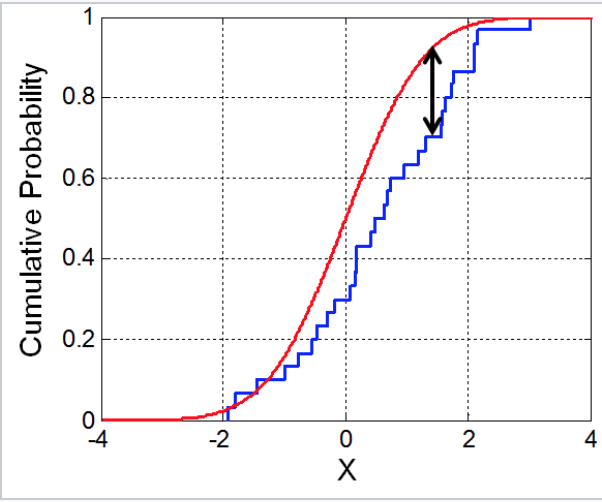
\includegraphics[width = .5\textwidth]{KS}
		\caption{Illustration of the KS statistic. The red curve is a theoretical CDF; the blue curve is an empirical CDF. The KS statistic is the size of the largest vertical distance between the two. Image source: \href{https://en.wikipedia.org/wiki/Kolmogorov-Smirnov\_test}{Wikipedia}.} \label{fig:KS}
	\end{figure}

	Our method to pick $k_{\text{min}}$ is simple -- we just choose $\hat{k}_{\text{min}} = \argmin D(k_{\text{min}}$; that is, the cutoff is chosen to minimize the KS statistic. In practice, this involves calculating $\hat{\gamma}$ for each possible value of $k_{\text{min}}$. Fortunately, Equation \eqref{eq:numerical} can be solved efficiently, so this process is computationally tractable. 

\section*{Model Evaluation}

	We now have optimal values of $\hat{\gamma}$ and $\hat{k}_{\text{min}}$ -- we have ``fit'' a power law to the data. But is our best power law model really a plausible explanation of the data? If the data is really exponential or log-normal, for example, even our best model will provide a poor explanation. How can we evaluate whether the power law fits? 

	For this task, we return to the KS statistic $D$. Recall that $D$ measures the largest discrepancy between the empirical CDF and theoretical CDF. Intuitively, if $D$ is large, then even our best model is ``not very good.'' But how large is large? What we need is an \emph{null distribution} on $D$ that tells us how \emph{likely} it is that $D$ would take a given value. To obtain this null distribution, we use bootstrapping: 
	\begin{enumerate}
		\item We draw $n$ samples from our theoretical distribution $p_K(k;\hat{\gamma}, \hat{k}_{\text{min}}$, and compute $\tilde{D}$ for this synthetic data set. 
		\item We repeat Step 1 many times, obtaining an \emph{bootstrap distribution} for   $\tilde{D}$. 
		\item We compare our empirical $D$ to the bootstrap distribution. Using the distribution, we can compute $p = \prob(\tilde{D} \geq D)$; i.e. the probability that the data would have KS statistic greater than or equal to what we observed, if it ``really'' came from our theoretical model. 
	\end{enumerate}
	We've labeled it $p$ for a reason -- this is a $p$-value. Unlike in many other contexts, note that large values of $p$ are ``good,'' in the sense tha they better support the power law hypothesis. In practice, it is common to take $p < 0.1$ to be evidence \emph{against} the hypothesis, and $p \geq 0.1$ to indicate that the data is \emph{consistent} with the hypothesis. 

\bibliography{/Users/phil/bibs/library.bib}{}
\bibliographystyle{apalike}

\end{document}